% !TeX program = pdflatex
% !TeX spellcheck = en_EN
% !TeX encoding = UTF-8
% !BIB program = biber


\documentclass[oneside,11pt,titlepage,a4paper,ngerman,bibliography=totocnumbered,listof=numbered, hidelinks]{scrbook}
%
% Template Style
% =========================================================================
% = IKM THESIS TEMPLATE STYLE
% =========================================================================

% www.ikm.tu-berlin.de
% ------------------------
% this template consists of various adaptions from different sources for non-profit use.

% Trotz angewandter Sorgfalt kann für die Richtigkeit, Vollständigkeit oder Aktualität dieser Vorlage keine
% Haftung übernommen werden. Die Technische Universität Berlin ist darüber hinaus nicht in der Lage, irgendeine
% Haftung für einen möglichen Schaden oder sonstige Konsequenzen zu tragen, die sich aus der direkten oder
% indirekten Verwendung der bereitgestellten Inhalte ergeben.

% Kontakt: Max Theilig TU Berlin (m.theilig@tu-berlin.de)


% =========================================================================
% = MISC
% =========================================================================

\usepackage{a4wide}					%
\usepackage{verbatim}				%
\usepackage[toc,page]{appendix}			%
\usepackage[nohyperlinks, withpage, smaller]{acronym}			% abbreviations
\usepackage{amsthm}				% Definitions


% =========================================================================
% = COLORS
% =========================================================================
% Make sure to use color only in absolutly necessary

\usepackage{xcolor}					% Colors
\definecolor{LightBlue}{rgb}{0.55,0.55,1}
\definecolor{DarkBlue}{rgb}{0.2,0.2,0.5}
\definecolor{DarkRed}{rgb}{0.71,0.12,0.07} % TU-Berlin red
\definecolor{IKMBlue}{RGB}{1,26,153} % IKM blue


% =========================================================================
% = PAGE LAYOUT
% =========================================================================

\usepackage{geometry}
\geometry{left=3.5cm, right=2.5cm, bottom=2.5cm,top=2.5cm}

\newcommand{\setwidesite}				% changes the geometry to have less margin
{
	\fancyhfoffset[LE,RO]{0cm}
	\fancyheadoffset[LO,RE]{0cm}
	\fancyfootoffset[RE]{2cm}
	\newgeometry{left=2.5cm, right=1.8cm, bottom=1.8cm,top=1.8cm}
}

\setlength{\parindent}{0mm}
%\setlength{\parindent}{4mm}
\setlength{\parskip}{1.5mm}
\newcommand{\forceindent}{\leavevmode{\parindent=4mm\indent}}


% =========================================================================
% = TYPESETTING
% =========================================================================

\usepackage[hyphens]{url}				% url
\usepackage{hyphenat}				% hyphenation. use \hyphenation{}

\righthyphenmin=5
\lefthyphenmin=5
% custom hyphenation					% add words to this list to prevent hyphenation
\hyphenation{
ASCII
TCP
}

% =========================================================================
% = TABLE OF CONTENTS
% =========================================================================

\setcounter{secnumdepth}{4}
\setcounter{tocdepth}{3}

\addtokomafont{disposition}{\rmfamily}

% =========================================================================
% = FONTS
% =========================================================================

\usepackage{mathpazo}	%palatino, palatino math
\usepackage[scaled=.95]{helvet} %san serif
\usepackage{courier} %typewriter

% Adding a finite stretch on the page suppresses "Underfull \vbox (badness 10000)" warnings.
\makeatletter
\def\@textbottom{\vskip \z@ \@plus 1pt}
\let\@texttop\relax
\makeatother

% =========================================================================
% = SYMBOLS
% =========================================================================

%\usepackage{gensymb}
\usepackage{textcomp} 				% for \textmu (non-italic $\mu$)
\makeatletter						% this makes "@" a regular letter


% =========================================================================
% = TABLES
% =========================================================================

\usepackage{tabularx}
\usepackage{booktabs}
\usepackage{multirow}
\usepackage{longtable}				% tables spanning over more than one page

%%\setlength{\fboxsep}{0mm}			% spacing between \fbox border and content

\usepackage{amsmath}				% math fonts
\usepackage{amssymb}				% math symbols
\usepackage[onehalfspacing]{setspace}				% 1.5 line spacing


% =========================================================================
% = BIBILOGRAPHY, REFERENCES
% =========================================================================


%make readable references
\usepackage[pdftex,pdfpagelabels=true]{hyperref}

\usepackage[style=apa,natbib=true,backend=biber,apabackref=true,backrefstyle=three+]{biblatex}

\bibliography{Bibliography}


% =========================================================================
% = LANGUAGE & ENCODING
% =========================================================================

\usepackage[ngerman]{babel}				% \usepackage[english]{babel}

\selectlanguage{ngerman}				% \selectlanguage{english}

\usepackage[T1]{fontenc}
%\usepackage[latin1]{inputenc}				% can use native umlauts
\usepackage[utf8]{inputenc}				% can use native umlauts

\usepackage[babel,german=quotes]{csquotes}	% provides \enquote{Blupp} => "`Blupp"'
%\usepackage[babel,english=american]{csquotes}	% provides \enquote{Blupp} => "`Blupp"'

\SetCiteCommand{\parencite}			% Changed for biblatex

\usepackage{units}					% unified way of setting values with units

\usepackage{appendix}

%to change to counter in the appendix, currently not used because a little more complex especially for listings
\usepackage{chngcntr}


%appendix does not support babel
\addto\captionsngerman{\let\appendixtocname\appendixname%
\let\appendixpagename\appendixname}

% =========================================================================
% = CODE LISTINGS
% =========================================================================

\usepackage{listings}

\renewcommand{\lstlistlistingname}{\lstlistingname{}sverzeichnis}

% Listings Styles from SNET TU-Berlin

\definecolor{violet}{cmyk}{0.45,0.97,0.27,0.21}
\definecolor{lstblue}{cmyk}{1,0.80,0,0}
\definecolor{lstgreen}{cmyk}{0.71,0.21,0.65,0.22}
\definecolor{bluegrey}{cmyk}{0.56,0.24,0.11,0.05}
\definecolor{javadoc}{cmyk}{0.88,0.59,0,0}
\definecolor{lstgrey}{cmyk}{0.55,0.44,0.42,0.32}

\lstdefinelanguage{SQL}{
     keywords={},
     keywordstyle=\color{bluegrey}\bfseries,
     morekeywords=[2]{CREATE,TABLE,IF,NOT,EXISTS,NULL,SET,DEFAULT,PRIMARY,KEY,COLLATE,CHARACTER,AUTO_INCREMENT,ENGINE,CHARSET},
     keywordstyle={[2]\color{violet}\bfseries},
     otherkeywords={int,varchar,double,text,tinyint},
     sensitive=false,
     morecomment=[l][\color{lstgreen}]{//},
     morecomment=[s][\color{lstgreen}]{/*}{*/},
     morecomment=[s][\color{javadoc}]{/**}{*/},
     morestring=[b]',
     morestring=[b]"
  }
\lstdefinelanguage{PHP}{
     keywords={},
     keywordstyle=\color{bluegrey}\bfseries,
     morekeywords=[2]{static,function,if,return,pow,sin,cos,asin,min,sqrt,int},
     keywordstyle={[2]\color{violet}\bfseries},
     otherkeywords={@param, @returns, @author, @type, @link, @see},
     sensitive=false,
     morecomment=[l][\color{lstgreen}]{//},
     morecomment=[s][\color{lstgreen}]{/*}{*/},
     morecomment=[s][\color{javadoc}]{/**}{*/},
     morestring=[b]',
     morestring=[b]"
  }
\lstdefinelanguage{JavaScript}{
     keywords={},
     keywordstyle=\color{bluegrey}\bfseries,
     morekeywords=[2]{attributes, class, classend, do, empty, endif, endwhile, fail, function, functionend, if, implements, in, inherit, inout, not, of, operations, out, return, set, then, types, while, use},
     keywordstyle={[2]\color{violet}\bfseries},
     otherkeywords={@param, @returns, @author, @type, @link, @see},
     sensitive=false,
     morecomment=[l][\color{lstgreen}]{//},
     morecomment=[s][\color{lstgreen}]{/*}{*/},
     morecomment=[s][\color{javadoc}]{/**}{*/},
     morestring=[b]',
     morestring=[b]"
  }
\lstdefinelanguage{Java}{
     keywords={},
     keywordstyle=\color{bluegrey}\bfseries,
     morekeywords=[2]{abstract,boolean,break,byte,case,catch,char,class,
      const,continue,default,do,double,else,extends,false,final,
      finally,float,for,goto,if,implements,import,instanceof,int,
      interface,label,long,native,new,null,package,private,protected,
      public,return,short,static,super,switch,synchronized,this,throw,
      throws,transient,true,try,void,volatile,while},
     keywordstyle={[2]\color{violet}\bfseries},
     morekeywords=[3]{@SuppressWarnings, @Capability, @Override},
     keywordstyle={[3]\color{lstgrey}},
     otherkeywords={@param, @return, @returns, @author, @link, @see},
     sensitive,
     morecomment=[l]//,
     morecomment=[s]{/*}{*/},
     morecomment=[s][\color{javadoc}]{/**}{*/},
     morestring=[b]",
     morestring=[b]',
  }[keywords,comments,strings]
  
% some listings styles from Gregor Aisch
% http://vis4.net/blog/2009/09/noch-mehr-sprach-definitionen-fuer-latex-listings/

\lstdefinelanguage{CPP} {morekeywords={BRIEFDescriptorConfig,string,TiXmlNode,DetectorDescriptorConfigContainer,istringstream,cerr,exit},
language=C++,
keywordstyle=\color{bluegrey}\bfseries,
keywordstyle={[2]\color{violet}\bfseries},
keywordstyle={[3]\color{lstgrey}}}

\lstdefinelanguage{HTML5}{morekeywords={a, abbr, address, area, article, aside, audio, b, base, bb, bdo, blockquote,  body, br, button, canvas, caption, cite, code, col, colgroup, command, datagrid, datalist, dd, del, details, dialog, dfn, div, dl, dt, em, embed, eventsource, fieldset, figure, footer,  form,  h1, h2,  h3,  h4, h5,  h6,  head,  header,  hr, html,  i, iframe,  img,  input,  ins, kbd,  label,  legend,  li,  link,  mark,  map,  menu,  meta,  meter,  nav,  noscript,  object,  ol,  optgroup,  option,  output,  p,  param,  pre,  progress,  q,  ruby,  rp,  rt,  samp,  script,  section,  select,  small,  source,  span,  strong,  style,  sub,  sup,  table,  tbody,  td,  textarea,  tfoot,  th,  thead,  time,  title,  tr,  ul,  var,  video},
sensitive=false, morecomment=[s]{<!--}{-->}, morestring=[b]", morestring=[d]'}

\lstdefinelanguage{CSS} {morekeywords={azimuth,  background-attachment,  background-color,  background-image,  background-position,  background-repeat,  background,  border-collapse,  border-color,  border-spacing,  border-style,  border-top, border-right, border-bottom, border-left,  border-top-color, border-right-color, border-bottom-color, border-left-color,  border-top-style, border-right-style, border-bottom-style, border-left-style,  border-top-width, border-right-width, border-bottom-width, border-left-width,  border-width,  border,  bottom,  caption-side,  clear,  clip,  color,  content,  counter-increment,  counter-reset,  cue-after,  cue-before,  cue,  cursor,  direction,  display,  elevation,  empty-cells,  float,  font-family,  font-size,  font-style,  font-variant,  font-weight,  font,  height,  left,  letter-spacing,  line-height,  list-style-image,  list-style-position,  list-style-type,  list-style,  margin-right, margin-left,  margin-top, margin-bottom,  margin,  max-height,  max-width,  min-height,  min-width,  orphans,  outline-color,  outline-style,  outline-width,  outline,  overflow,  padding-top, padding-right, padding-bottom, padding-left,  padding,  page-break-after,  page-break-before,  page-break-inside,  pause-after,  pause-before,  pause,  pitch-range,  pitch,  play-during,  position,  quotes,  richness,  right,  speak-header,  speak-numeral,  speak-punctuation,  speak,  speech-rate,  stress,  table-layout,  text-align,  text-decoration,  text-indent,  text-transform,  top,  unicode-bidi,  vertical-align,  visibility,  voice-family,  volume,  white-space,  widows,  width,  word-spacing,  z-index},
sensitive=false, morecomment=[s]{/*}{*/}, morestring=[b]", morestring=[d]'}

\lstdefinelanguage{JavaFX} {morekeywords={abstract, after, and, as, assert, at, attribute, before, bind, bound, break, catch, class, continue, def, delete, else, exclusive, extends, false, finally, first, for, from, function, if, import, indexof, in, init, insert, instanceof, into, inverse, last, lazy, mixin, mod, new, not, null, on, or, override, package, postinit, private, protected, public-init, public, public-read, replace, return, reverse, sizeof, static, step, super, then, this, throw, trigger, true, try, tween, typeof, var, where, while, with },
sensitive=false, morecomment=[l]{//}, morecomment=[s]{/*}{*/}, morestring=[b]", morestring=[d]'}

\lstdefinelanguage{MXML} {morekeywords={mx:Accordion, mx:Box, mx:Canvas, mx:ControlBar, mx:DividedBox, mx:Form, mx:FormHeading, mx:FormItem, mx:Grid, mx:GridItem, mx:GridRow, mx:HBox, mx:HDividedBox, mx:LinkBar, mx:Panel, mx:TabBar, mx:TabNavigator, mx:Tile, mx:TitleWindow, mx:VBox, mx:VDividedBox, mx:ViewStack, mx:Button, mx:CheckBox, mx:ComboBase, mx:ComboBox, mx:DataGrid, mx:DateChooser, mx:DateField, mx:HRule, mx:Image, mx:Label, mx:Link, mx:List, mx:Loader, mx:MediaController, mx:MediaDisplay, mx:MediaPlayback, mx:MenuBar, mx:NumericStepper, mx:ProgressBar, mx:RadioButton, mx:RadioButtonGroup, mx:Spacer, mx:Text, mx:TextArea, mx:TextInput, mx:Tree, mx:VRule, mx:VScrollBar, mx:Application, mx:Repeater, mx:UIComponent, mx:UIObject, mx:View, mx:FlexExtension, mx:UIComponentExtension, mx:UIObjectExtension, mx:Fade, mx:Move, mx:Parallel, mx:Pause, mx:Resize, mx:Sequence, mx:WipeDown, mx:WipeLeft, mx:WipeRight, mx:WipeUp, mx:Zoom, mx:EventDispatcher, mx:LowLevelEvents, mx:UIEventDispatcher, mx:CurrencyFormatter, mx:DateFormatter, mx:NumberFormatter, mx:PhoneFormatter, mx:ZipCodeFormatter, mx:CursorManager, mx:DepthManager, mx:DragManager, mx:FocusManager, mx:HistoryManager, mx:LayoutManager, mx:OverlappedWindows, mx:PopUpManager, mx:SystemManager, mx:TooltipManager, mx:CreditCardValidator, mx:DateValidator, mx:EmailValidator, mx:NumberValidator, mx:PhoneNumberValidator, mx:SocialSecurityValidator, mx:StringValidator, mx:ZipCodeValidator, mx:DownloadProgressBar, mx:ArrayUtil, mx:ClassUtil, mx:Delegate, mx:ObjectCopy, mx:URLUtil, mx:XMLUtil, mx:CSSSetStyle, mx:CSSStyleDeclaration, mx:CSSTextStyles, mx:StyleManager, mx:HTTPService, mx:RemoteObject, mx:Service},
sensitive=false, morecomment=[s]{<!--}{-->}, morestring=[b]", morestring=[d]'}

\lstdefinelanguage{LZX} {morekeywords={a, alert, animator, animatorgroup , attribute, audio , axis, axisstyle , b, barchart, basebutton , basebuttonrepeater , basecombobox , basecomponent , basedatacombobox , basedatepicker , basedatepickerday , basedatepickerweek , basefloatinglist , basefocusview , baseform , baseformitem , basegrid , basegridcolumn , baselist , baselistitem , basescrollarrow , basescrollbar , basescrollthumb , basescrolltrack , baseslider , basestyle , basetab , basetabelement , basetabpane , basetabs , basetabsbar , basetabscontent , basetabslider , basetrackgroup , basetree , basevaluecomponent , basewindow , br , button , canvas , chart , chartbgstyle , chartstyle , checkbox , class , columnchart , combobox , command , connection , connectiondatasource , constantboundslayout , constantlayout , datacolumn , datacombobox , datalabel , datamarker , datapath , datapointer , dataselectionmanager , dataseries , dataset , datasource , datastyle , datastylelist , datatip , datepicker , debug , dragstate , drawview , edittext , event , face , floatinglist , font , font , form , frame , grid , gridcolumn , gridtext , handler , hbox , horizontalaxis , hscrollbar , i , image , img , import , include , inputtext , javarpc , label , labelstyle , layout , legend , library , linechart , linestyle , list , listitem , LzTextFormat , menu , menubar , menuitem , menuseparator , method , modaldialog , multistatebutton , node , p , param , piechart , piechartplotarea , plainfloatinglist , plotstyle , pointstyle , pre , radiobutton , radiogroup , rectangularchart , regionstyle , remotecall , resizelayout , resizestate , resource , reverselayout , richinputtext , rpc , script , scrollbar , security , selectionmanager , sessionrpc , simpleboundslayout , simpleinputtext , simplelayout , slider , soap , splash , stableborderlayout , state , statictext , style , submit , swatchview , SyncTester , tab , tabelement , tabpane , tabs , tabsbar , tabscontent , tabslider , Test , TestCase , TestResult , TestSuite , text , textlistitem , tickstyle , tree , u , valueline , valuelinestyle , valuepoints , valuepointstyle , valueregion , valueregionstyle , vbox , verticalaxis , view , view , vscrollbar , webapprpc , window , windowpanel , wrappinglayout , XMLHttpRequest , xmlrpc , zoomarea},
sensitive=false, morecomment=[s]{<!--}{-->}, morestring=[b]", morestring=[d]'}

\lstset{
  numbers=left,
  numberstyle=\tiny,
  numbersep=5pt,
  breaklines=true,
  stepnumber=1,
  tabsize=2,
  basicstyle=\ttfamily\small,
  frame=none,
  numberfirstline=true,
  firstnumber=1,
  keywordstyle=\color{violet}\bfseries,
  ndkeywordstyle=\color{bluegrey}\bfseries,
  identifierstyle=\color{black},
  commentstyle=\color{lstgreen}\ttfamily,
  stringstyle=\color{lstblue}\ttfamily,
  showstringspaces=false
}


% ========================================================================
% = CHANGE LIST DEFINITIONS
% ========================================================================

% order of item list
\renewcommand{\labelitemi}{$\bullet$}
\renewcommand{\labelitemii}{$\circ$}
\renewcommand{\labelitemiii}{$\ast$}
\renewcommand{\labelitemiv}{$\diamond$}

% order of enum list
\renewcommand{\labelenumi}{\arabic{enumi}.}
\renewcommand{\labelenumii}{\alph{enumii})}
\renewcommand{\labelenumiii}{\roman{enumiii}.}
\renewcommand{\labelenumiv}{\Alph{enumiv}.}


% ========================================================================
% = FOOTNOTES
% ========================================================================

% change color of footnotes
% \renewcommand{\thefootnote}{\color{DarkRed}\arabic{footnote}}

% use nice footnote indentation
\deffootnote[1em]{1em}{1em}{\textsuperscript{\thefootnotemark}\,}


% =========================================================================
% = GRAPHICS AND IMAGES
% =========================================================================

\usepackage{graphicx}
\graphicspath{{images/}}				% path to your image folder

\usepackage{eso-pic}					% needed for the full-face titlepage
\usepackage{chngpage}				% we need this to determine if a figure is on an odd or even page
\usepackage{tikz}					% tikz pictures

% captions of tables and images
\usepackage[hang,small,sf]{caption}
\renewcommand{\captionfont}{\sffamily\small}
\renewcommand{\captionlabelfont}{\bfseries}

\usepackage{float}
\usepackage{placeins}
% \floatstyle{ruled}
%\floatplacement

\renewcommand{\floatpagefraction}{0.85}		% if a figure takes more than 85% of a page it will be typeset on a separate page
\usepackage[it,bf,tight,hang,raggedright]{subfigure}

%\numberwithin{figure}{section}
%\numberwithin{table}{section}


% =========================================================================
% = HEADER
% =========================================================================

\newcommand{\STYLEfootnotetext}
{
  \begin{minipage}
  {.2\textwidth}
    \includegraphics[width=0.9\textwidth]{images/snet/snet_footer.png}
  \end{minipage}
}

% Change page headers and footers:
\usepackage{calc}
\usepackage{fancyhdr}
\pagestyle{fancy}
\fancyhfoffset[RO,LE]{0.1cm} %{\marginparsep+\marginparwidth}
\fancyhfoffset[RE,LO]{0.1cm}
%\fancyheadoffset[RE,LO]{\hoffset + \oddsidemargin}
\renewcommand{\headrule}{{%
%\color{DarkRed}%
%\color{IKMBlue}%
  \hrule width\headwidth height\headrulewidth \vskip-\headrulewidth}}
\fancyhf{}
\fancyhead[RE]{\slshape \nouppercase{\leftmark}}    % Even page header: "page   chapter"
\fancyhead[LO]{\slshape \nouppercase{\rightmark}}   % Odd  page header: "section   page"
\fancyhead[RO,LE]{\bfseries \thepage}

%- \fancyfoot[LE]{\STYLEleftpicture}
%- \fancyfoot[RO]{\STYLErightpicture}
\fancyfoot[LE]{\STYLEfootnotetext}

\renewcommand{\headrulewidth}{1pt}    % Underline headers
\renewcommand{\footrulewidth}{0pt}

% =========================================================================
% = SECTIONS THEMING
% =========================================================================

\newcommand{\allsectionformat}{%
%\color{DarkRed}%
%\color{IKMBlue}%
\rmfamily\normalfont}

% Font style and colors
\addtokomafont{part}{\Huge\allsectionformat}
\addtokomafont{chapter}{\Huge\allsectionformat}
\addtokomafont{section}{\allsectionformat}
\addtokomafont{subsection}{\allsectionformat}
\addtokomafont{subsubsection}{\allsectionformat}
\addtokomafont{paragraph}{\allsectionformat}
\addtokomafont{subparagraph}{\allsectionformat}

% Spacing before and after the section titles
\RedeclareSectionCommand[
  beforeskip=-.75\baselineskip,
  afterskip=.5\baselineskip]{section}

\RedeclareSectionCommand[
  beforeskip=-5\baselineskip,
  afterskip=.5\baselineskip]{chapter}


% =========================================================================
% = TYPESETTING - TWEAKES
% =========================================================================

\addtokomafont{section}{\LARGE}
\addtokomafont{subsection}{\large}

% instead of sloppy
%\tolerance 1414
%\hbadness 1414
%- \tolerance 2414
%- \hbadness 2414
%- \emergencystretch 1.5em
%- \hfuzz 0.3pt
%- \widowpenalty=10000     % Hurenkinde r
%- \clubpenalty=10000      % Schusterjungen
%- \brokenpenalty=10000
%- \interlinepenalty=9000 % seitenumbruch im absatz
%- \vfuzz \hfuzz
%- \raggedbottom


% =========================================================================
% =  USER DEFINED COMMANDS
% =========================================================================

\newcommand{\chapterquote}[2]{
    \begin{quotation}
    \begin{flushright}
    \noindent\emph{``{#1}''\\[1.5ex]---{#2}}
    \end{flushright}
    \end{quotation}
}

\addbibresource{bibliography.bib}

\usepackage{todonotes}

\begin{document}

%--------------------------------------------------------------
% FRONT PAGE AND DOCUMENT METADATA
%--------------------------------------------------------------
%Metadata
\hypersetup{%
	draft=false,
	pdftitle={European Code Hub},
	pdfauthor={Patrick Reuter},
	pdfkeywords={key1, key2, key3},
	pdfsubject={Thesis Subject}
}

\frontmatter

%\begin{titlepage}	
\noindent
\begin{minipage}{0.75\textwidth}
{\small
Technische Universit\"at Berlin\\
Fakult\"at VII - Wirtschaft und Management\\
Fachbereich Informations- und Kommunikationsmanagement\\
Prof. Dr. Rüdiger Zarnekow\\
}%
\end{minipage}%
\begin{minipage}{0.25\textwidth}%
\begin{figure}[H]%
{\raggedleft
\includegraphics[height=2cm]{images/TU_Logo_lang_RGB_rot.png}}
\end{figure}%
\hfill
\end{minipage}%

\vspace{2cm}

\thispagestyle{empty}
\begin{center}

{\large
A proposal submitted in fulfillment of the requirements\\
Degree of Master of Science in Information Systems Management}\\
\vspace{1cm}
{\huge\textbf
European Code Hub:\\
Establishing Collaboration in the European Union through an Open Source Code Platform
}
\vspace{1.2cm}

{\large by\\
	 Patrick Reuter \\
	 Matriculation number: 358939\\[2cm]
}

\begin{minipage}{\linewidth} 
\begin{tabbing}
  		Reviewer:\quad \= Prof. Dr. Rüdiger Zarnekow, TU Berlin\\
                    \> Prof. Dr. Odej Kao, TU Berlin \\[0.3cm]
    	Supervisor:             \> Jakob Korbel, TU Berlin \\
    						         
\end{tabbing}
\end{minipage}

\vspace{1.5cm}
\today\todo{Check the date format} \\
\end{center}
\thispagestyle{empty}
\newpage
\setcounter{page}{1}
\end{titlepage}

% Clear two pages after the title
\shipout\null

%\chapter*{\LARGE Statutory Declaration}
I hereby declare that I have created this work completely on my own and used no other sources or tools than the ones listed.
\vspace{2em}

\noindent

\vspace{30 mm}
\begin{flushright}

\rule{90mm}{1pt}

Berlin, \today \hspace{15 mm} Patrick Reuter
\end{flushright}

%\chapter*{Acknowledgments}
\label{cha:acknowledgments}

I would like to thank my teddybear...

%\chapter*{Abstract}
\label{cha:abstract}

In this thesis, we show that lorem ipsum dolor sit amet.					% EN Abstract
%\chapter{Zusammenfassung}
\label{cha:zusammenfassung}

Hier kommt das deutsche Abstract hin. Wie das geht, kann man wie immer auf Wikipedia nachlesen \url{http://de.wikipedia.org/wiki/Abstract}...	% DE Abstract


\tableofcontents{}

%--------------------------------------------------------------
% TABLES, FIGURES, ABBREVIATIONS
%--------------------------------------------------------------
\backmatter

% Lists of tables and figures
%\listoftables
%\listoffigures
%\lstlistoflistings
%\chapter{Abkürzungsverzeichnis}
\begin{acronym}[ECU]
\acro{ecu}[ECU]{European currency unit}
\acro{eu}[EU]{Europäische Union}
\acro{bse}[BSE]{Bovine spongiforme Enzephalopathie}
\end{acronym}

%--------------------------------------------------------------
% MAIN CONTENT
%--------------------------------------------------------------
\mainmatter

\chapter{Einleitung}
\label{cha:Einleitung}

\chapterquote{640K ought to be enough for anybody.}{William Henry Gates III, on a sunny day, 1981}

\forceindent Lorem ipsum \citep{FakePaper11} dolor \footnote{Fußnoten sollen auf derselben Seite wie die Textstelle stehen, auf die sie sich beziehen, und sind fortlaufend sowie lückenlos zu nummerieren} kasd gubergren, no sea takimata sanctus est Lorem ipsum dolor sit amet. Lorem ipsum dolor sit amet, consetetur sadipscing el.

\textbf{Bitte beachten} Sie neben \textcite{book} auch das Dokument \enquote{typographie.pdf} in der Ordnerstruktur.

nonumy eirmod tempor invidunt ut labore et dolore magna aliquyam erat, sed diam voluptua. At vero eos et accusam et justo duo dolores et ea rebum. Stet clita kasd gubergren, no sea takimata sanctus est Lorem ipsum dolor sit amet. Lorem ipsum dolor sit amet, consetetur sadipscing elitr, sed diam nonumy eirmod tempor invidunt ut labore et dolore magna aliquyam erat, sed diam voluptua. At vero eos et accusam et justo duo dolores et ea rebum. Stet clita kasd gubergren, no sea takimata sanctus est Lorem ipsum dolor sit amet.
\lstset{language=JavaScript}
\begin{lstlisting}[caption=high skilled at javascript, label=hsj]
<!DOCTYPE HTML>
<html>

<body>

  <p>Before the script...</p>

  <script>
    alert( 'Hello, world!' );
  </script>

  <p>...After the script.</p>

</body>

</html>
\end{lstlisting}
Lorem ipsum dolor sit amet, consetetur sadipscing elitr, sed diam nonumy eirmod tempor invidunt ut labore et dolore magna aliquyam erat, sed diam voluptua. At vero eos et accusam et justo duo dolores et ea rebum. Stet clita kasd gubergren, no sea takimata sanctus est Lorem ipsum dolor sit amet.
Duis autem vel eum iriure dolor in hendrerit in vulputate velit esse molestie consequat, vel illum dolore eu feugiat nulla facilisis at vero eros et accumsan et iusto odio dignissim qui blandit praesent luptatum zzril delenit augue duis dolore te feugait nulla facilisi. Lorem ipsum dolor sit amet, consectetuer adipiscing elit, sed diam nonummy nibh euismod tincidunt ut laoreet dolore magna aliquam erat volutpat.

\begin{figure}[!ht]
	\centering
	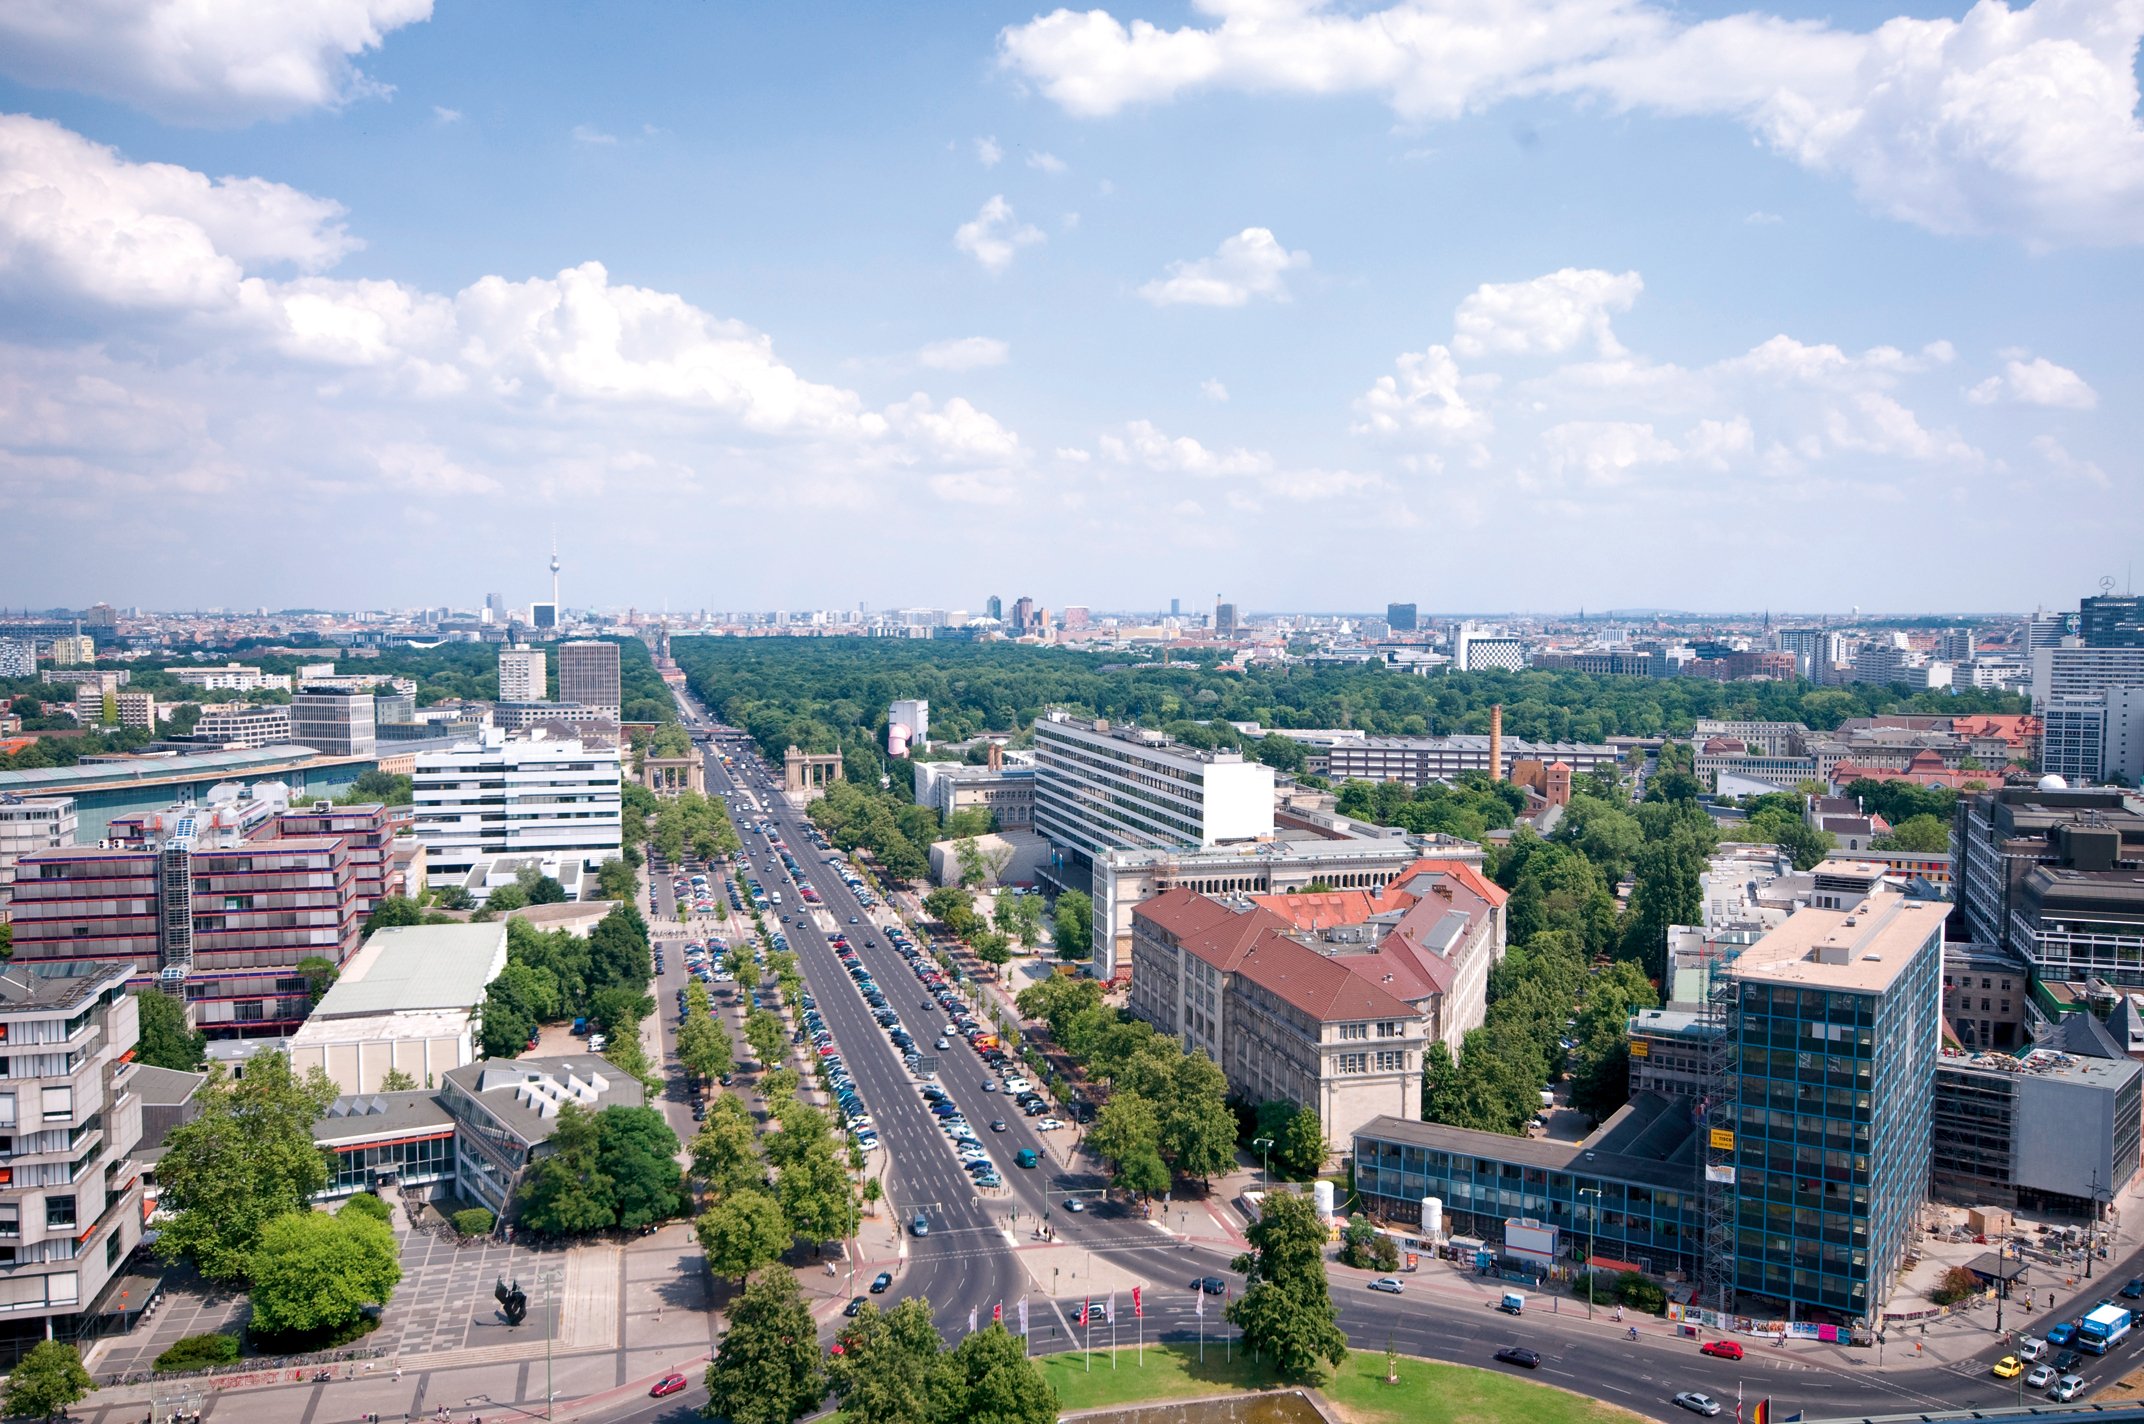
\includegraphics[width=0.9\textwidth]{images/TU_Bild-Aussicht_RGB.jpg}\\
	\caption{Images can be loaded from the images folder and sub folders}
	\label{fig:introduction__loremipsum}
\end{figure}

Ut wisi enim ad minim veniam, quis nostrud exerci tation ullamcorper suscipit lobortis nisl ut aliquip ex ea commodo consequat. Duis autem vel eum iriure dolor in hendrerit in vulputate velit esse molestie consequat, vel illum dolore eu feugiat nulla facilisis at vero eros et accumsan et iusto odio dignissim qui blandit praesent luptatum zzril delenit augue duis dolore te feugait nulla facilisi.\\
Nam liber tempor cum soluta nobis eleifend option congue nihil imperdiet doming id quod mazim placerat facer possim assum. Lorem ipsum dolor sit amet, consectetuer adipiscing elit, sed diam nonummy nibh euismod tincidunt ut laoreet dolore magna aliquam erat volutpat. Ut wisi enim ad minim veniam, quis nostrud exerci tation ullamcorper suscipit lobortis nisl ut aliquip ex ea commodo consequat.

Duis autem vel eum iriure dolor in hendrerit in vulputate velit esse molestie consequat, vel illum dolore eu 

At vero eos et accusam et justo duo dolores et ea rebum. Stet clita kasd gubergren, no sea takimata sanctus est Lorem ipsum dolor sit amet. Lorem ipsum dolor sit amet, consetetur sadipscing elitr, sed diam nonumy eirmod tempor invidunt ut labore et dolore magna aliquyam erat, sed diam voluptua. At vero eos et accusam et justo duo dolores et ea rebum. Stet clita kasd gubergren, no sea takimata sanctus est Lorem ipsum dolor sit amet. Lorem ipsum dolor sit amet, consetetur sadipscing elitr, At accusam aliquyam diam diam dolore dolores duo eirmod eos erat, et nonumy sed tempor et et invidunt justo labore Stet clita ea et gubergren, kasd magna no rebum. sanctus sea sed takimata ut vero voluptua. est Lorem ipsum dolor sit amet. Lorem ipsum dolor sit amet, consetetur

\section{Lorem ipsii}

Lorem ipsum dolor sit amet, consetetur sadipscing elitr, sed diam nonumy eirmod tempor invidunt ut labore et dolore magna aliquyam erat, sed diam voluptua. At vero eos et accusam et justo duo dolores et ea rebum. Stet clita kasd gubergren, no sea takimata sanctus est Lorem ipsum dolor sit amet. Lorem ipsum dolor sit amet, consetetur sadipscing elitr, sed diam nonumy eirmod tempor invidunt ut labore et dolore magna aliquyam erat, sed diam voluptua. At vero eos et accusam et justo duo dolores et ea rebum. Stet clita kasd gubergren, no sea takimata sanctus est Lorem ipsum dolor sit amet. Lorem ipsum dolor sit amet, consetetur sadipscing elitr, sed diam nonumy eirmod tempor invidunt ut labore et dolore magna aliquyam erat, sed diam voluptua. At vero eos et accusam et justo duo dolores et ea rebum. Stet clita kasd gubergren, no sea takimata sanctus est Lorem ipsum dolor sit amet.

\begin{table}[!ht]
	\small
	\centering
	\begin{tabular}{|l|l|l|l|}
		\hline
		Lorem & ipsum & dolor & sit \\
		\hline
		amet & consetetur & sadipscing & elitr \\
		\hline
		Lorem & ipsum & dolor & sit \\
		\hline
		amet & consetetur & sadipscing & elitr \\
		\hline
	\end{tabular}
	\caption{Lorem ipsum...}
\end{table}

Duis autem vel eum iriure dolor in hendrerit in vulputate velit esse molestie consequat, vel illum dolore eu feugiat nulla facilisis at vero eros et accumsan et iusto odio dignissim qui blandit praesent luptatum zzril delenit augue duis dolore te feugait nulla facilisi. Lorem ipsum dolor sit amet, consectetuer adipiscing elit, sed diam nonummy nibh euismod tincidunt ut laoreet dolore magna aliquam erat volutpat.

\subsection{Lorem ipsum continued}

Ut wisi enim ad minim veniam, quis nostrud exerci tation ullamcorper suscipit lobortis nisl ut aliquip ex ea commodo consequat. Duis autem vel eum iriure dolor in hendrerit in vulputate velit esse molestie consequat, vel illum dolore eu feugiat nulla facilisis at vero eros et accumsan et iusto odio dignissim qui blandit praesent luptatum zzril delenit augue duis dolore te feugait nulla facilisi.

\subsubsection{Even more Lorem Ipsii}

Nam liber tempor cum soluta nobis eleifend option congue nihil imperdiet doming id quod mazim placerat facer possim assum. Lorem ipsum dolor sit amet, consectetuer adipiscing elit, sed diam nonummy nibh euismod tincidunt ut laoreet dolore magna aliquam erat volutpat. Ut wisi enim ad minim veniam, quis nostrud exerci tation ullamcorper suscipit lobortis nisl ut aliquip ex ea commodo consequat.

Duis autem vel eum iriure dolor in hendrerit in vulputate velit esse molestie consequat, vel illum dolore eu feugiat nulla facilisis.

At vero eos et accusam et justo duo dolores et ea rebum. Stet clita kasd gubergren, no sea takimata sanctus est Lorem ipsum dolor sit amet. Lorem ipsum dolor sit amet, consetetur sadipscing elitr, sed diam nonumy eirmod tempor invidunt ut labore et dolore magna aliquyam erat, sed diam voluptua. At vero eos et accusam et justo duo dolores et ea rebum. Stet clita kasd gubergren, no sea takimata sanctus est Lorem ipsum dolor sit amet. Lorem ipsum dolor sit amet, consetetur sadipscing elitr, At accusam aliquyam diam diam dolore dolores duo eirmod eos erat, et nonumy sed tempor et et invidunt justo labore Stet clita ea et gubergren, kasd magna no rebum. sanctus sea sed takimata ut vero voluptua. est Lorem ipsum dolor sit amet. Lorem ipsum dolor sit amet, consetetur.

\chapter{Theoretical foundations}
\label{cha:theoretical_foundations}

Introduction, motivation, reasons to do this...

\section{Open Source}

Let's write some cool stuff about Open Source...


\subsection{Open Source Code}

Let's write some cool stuff about Open Source...

\subsection{Open Source Licences}

Let's write some cool stuff about Open Source...

\subsection{Github}

Let's write some cool stuff about Github...

\subsection{Economical comparison between Open Source and Licensing Models}

Don't write too much about Economical comparison between Open Source and Licensing Models...
\section{European Union}

Let's write some cool stuff about Open Source...


\subsection{Political position}
\subsection{Public money is public code initiative}
\subsection{Digitization and uprising of domestic Digital Service Agencies}

- Government Digital Service in the United Kingdom
- Digital Transformation Team Italy
\section{Best practices for Open Source Code platforms}

Let's write some cool stuff about Open Source...

\subsection{United States of America}

Something about USA...
- Code.gov
- Code.mil
- Code California


\subsection{Canada}

Something about Canada... Open Resource Exchange
\section{Open Source code platforms in the European Union}


Something about Opensourceprojects.eu and other stuff...
\chapter{Methodology of Design Science Research}
\label{cha:methodology_of_design_science_research}


Introduction, motivation, reasons to do this...
\chapter{Design Science Research}
\label{cha:design_science_research}

Introduction, motivation, reasons to do this...

\section{Problem identification}

Let's write some cool stuff about problems...
\section{Requirement to the solution}

Let's write some cool stuff about problems...


\subsection{Platform features}

Let's write some cool stuff about features...

\subsection{Data sources}

Data stuff...

\subsection{Estimated number of users}

Number of users...
\section{Design and development}

Let's write some cool stuff about problems...


\subsection{System architecture}

Architecture stuff

\subsection{Client-side}

Client...

\subsection{Server-side}

Server\dots

\subsection{Deployment}

Deployment\dots

\subsection{Evaluation}
\section{Evaluation}

Do some evaluation...


\subsection{Methodology}

Architecture stuff

\subsection{Results}

Client...

\subsection{Discussion}

Server\dots
\chapter{Conclusion}
\label{cha:conclusion}

Die Auswertung der Arbeit und deren Ergebnisse hier.

\section{Key findings}

Let's write some cool stuff about problems...
\section{Outlook}

Outlook....

%--------------------------------------------------------------
% BIBLOGRAPHY AND APPENDICES
%--------------------------------------------------------------
\backmatter


% Bibliography
\setwidesite{}						% Set page to be wider for bibliography
\markboth{Bibliography}{Bibliography}
\label{cha:bibliography}
\printbibliography

% Use following to separate online (websites) and offline (books, papers) sources
%\printbibliography[heading=offline,filter=offline]
%\printbibliography[heading=online,filter=online]

% \begin{appendices}
% 	\chapter{Anhang 1}
\label{appendix:listing1}

\lstset{language=PHP}
\begin{lstlisting}[caption={Additional Code},nolol]
for($i=1; $i<123; $i++)
{
    echo "latex is fun! ;)";
}
\end{lstlisting}
% 	% \input{content/99_appendices/a02_listings}
% 	% \input{content/99_appendices/a03_listings}
% \end{appendices}

\end{document}
